\documentclass{article}
 
\usepackage{pgf}
\usepackage{tikz}
\usetikzlibrary{arrows, decorations.pathmorphing, backgrounds, positioning, fit, petri, automata}
 
\definecolor{yellow1}{rgb}{1,0.8,0.2} 
 
%opening
\begin{document}
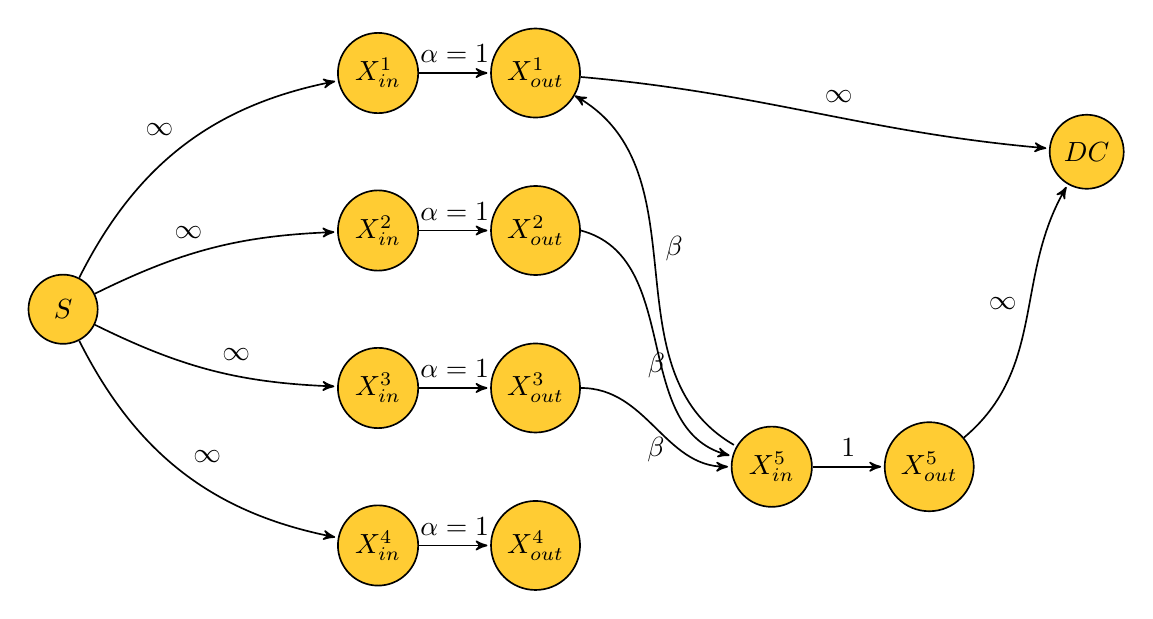
\begin{tikzpicture}[->,>=stealth',shorten >=1pt,auto,node distance=2.8cm,
                    semithick]
  \tikzstyle{every state}=[fill=yellow1,draw,text=black]
 
  \node[state]         (S) at (-6, 0)              {$S$};
  \node[state]         (xin1) at (-2, 3)           {$X^1_{in}$};
  \node[state]         (xin2) at (-2, 1)        {$X^2_{in}$};
  \node[state]         (xin3) at (-2, -1)       {$X^3_{in}$};
  \node[state]         (xin4) at (-2, -3)           {$X^4_{in}$};
  \node[state]         (xout1) at (0, 3)          {$X^1_{out}$};
  \node[state]         (xout2) at (0, 1)        {$X^2_{out}$};
  \node[state]         (xout3) at (0, -1)   {$X^3_{out}$};
  \node[state]         (xout4) at (0, -3)           {$X^4_{out}$};
  \node[state]         (xin5)  at (3, -2)   {$X^5_{in}$};
  \node[state]         (xout5) at (5, -2)   {$X^5_{out}$};
  \node[state]         (DC) at (7, 2)           {$DC$};
 
  \path (S) edge[bend left=26]              node {$\infty$} (xin1)
            edge[bend left=12]              node {$\infty$} (xin2)
            edge[bend right=12]             node {$\infty$} (xin3)
            edge[bend right=26]             node {$\infty$} (xin4)
        (xin1) edge  node {$\alpha=1$} (xout1)
        (xin2) edge  node {$\alpha=1$} (xout2)
        (xin3) edge  node {$\alpha=1$} (xout3)
        (xin4) edge  node {$\alpha=1$} (xout4)
        (xin5) edge  node {$1$} (xout5);
  \draw[<-] (xout1) to[out=-30,in=150] node {$\beta$} (xin5);
  \draw[->] (xout2.east) to[out=-15,in=165] node [below] {$\beta$} (xin5);
  \draw[->] (xout3.east) to[out=0,in=180] node [below] {$\beta$} (xin5.west);
  \draw[->] (xout1) to[out=-5,in=175] node {$\infty$} (DC);
  \draw[->] (xout5) to[out=40, in=-120] node {$\infty$} (DC);
\end{tikzpicture}












\end{document}